\chapter{\ResearchOneTitle}
\label{rq1:chapter}

本章针对机载通信能量受限且拓扑动态变化的无人机网络，研究路由与发射功率联合控制问题，旨在提升网络聚合吞吐量的同时延长网络可用寿命。如图~\ref{rq1:fig:scenario} 所示，每个节点在转发数据时需同步确定下一跳中继与对应发射功率：两者共同决定了链路传输速率与通信能耗，必须结合实时信道状态、邻居位置及剩余电量加以权衡。

\begin{figure}[!htbp]
  \centering
  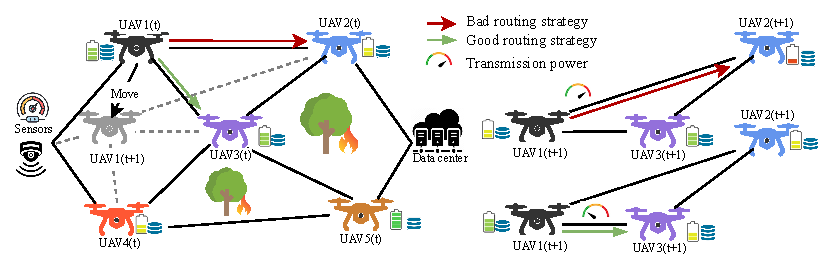
\includegraphics[width=0.96\textwidth]{figures/rq1/scenario.pdf}
  \bicaption{无人机集群中的多跳通信与能量感知路由场景}{Multi-hop communication and energy-aware routing in a UAV swarm}
  \label{rq1:fig:scenario}
\end{figure}

为此，本章提出一种基于李雅普诺夫优化的能量感知分布式路由方法 LEADR。该方法将数据队列积压、节点累计能耗及虚拟能量队列共同纳入逐时隙优化目标，在固定观测干扰下求得各候选链路发射功率的闭式解；随后结合邻居剩余能量与地理进度筛选下一跳，并依据节点相对运动速度自适应调整邻居探测（HELLO）消息的广播周期。下文依次阐述系统建模、算法设计与仿真评估，重点考察不同节点规模、通信范围及飞行速度下，LEADR 在转发性能与网络续航之间的权衡效果。

\section{系统模型与问题描述}
\label{rq1:sec:model}

\subsection{网络与链路模型}

考虑由 $N$ 架无人机（节点集合记为 $\mathcal{N}=\{1,2,\ldots,N\}$）与一个地面数据中心 $D$ 构成的多跳网络，无人机将采集的观测数据经一跳或多跳转发至中心。将总任务时长 $T$ 均匀划分为 $K$ 个决策时隙，时隙长度 $\Delta t=T/K$，索引记为 $t=0,1,\ldots,K-1$。

假设各无人机在固定高度飞行，其二维平面位置与速度向量分别记为 $\bm q_i(t)\in\mathbb{R}^{2}$ 和 $\bm v_i(t)\in\mathbb{R}^{2}$，任意两节点间的距离为
\begin{equation}
 d_{ij}(t)=\|\bm q_i(t)-\bm q_j(t)\|_2.
 \label{rq1:eq:distance}
\end{equation}
在最大通信范围 $R$ 内，节点 $i$ 当前活跃的邻居集合定义为
\begin{equation}
 \mathcal{N}_i(t)=\{j\in\mathcal{N}\setminus\{i\}:d_{ij}(t)\le R,\ E_j(t)>0\}.
 \label{rq1:eq:neighbors}
\end{equation}
若数据中心 $D$ 处于通信范围内，则直接纳入候选转发集合；数据中心不受机载电量限制，且只接收不转发。

无人机移动遵循高斯--马尔可夫（Gauss--Markov）模型，节点速度具有一定时间相关性，邻居拓扑随相对运动平滑演化。飞行轨迹由上层巡检任务预先给定，路由协议仅根据观测到的位置与速度信息进行通信调度。各节点通过周期性交换 HELLO 消息共享节点标识、时间戳、位置、速度、剩余电量及队列信息，借此维护本地邻居表并及时清理超时或预测失联的条目。本章主要符号汇总于表~\ref{rq1:tab:notation}。

\begin{table}[!htbp]
\centering\small
\bicaption{能量均衡路由模型的主要符号}{Main notation of the energy-balanced routing model}
\label{rq1:tab:notation}
\begin{tabularx}{\textwidth}{lX}
\toprule
符号 & 含义 \\
\midrule
$\mathcal{N},\mathcal{N}_i(t)$ & 无人机集合及节点 $i$ 在时隙 $t$ 的邻居集合 \\
$T,K,\Delta t$ & 任务持续时间、时隙数与决策间隔 \\
$\bm q_i(t),\bm v_i(t)$ & 节点位置与速度向量 \\
$d_{ij}(t),R$ & 节点间距离与通信范围 \\
$x_{ij}(t),p_{ij}(t)$ & 下一跳选择指示量与链路发射功率 \\
$h_{ij}(t),I_{ij}(t)$ & 链路增益与接收端并发干扰 \\
$r_{ij}(t),\mu_i(t),\nu_i(t)$ & 链路速率、节点服务速率与数据到达速率 \\
$Q_i(t),Q_{\max}$ & 数据积压与缓存容量上限 \\
$E_i(t),E_{\max}$ & 剩余通信能量与初始通信能量预算 \\
$\Phi_i(t),F_i(t)$ & 累计能量损耗与虚拟能量队列 \\
$\beta,\gamma,V$ & 能量损耗、预算偏差与吞吐收益的控制权重 \\
$W_{ij}(t),W_{ij}^{E,G}(t)$ & 基础链路权重与能量、地理修正后的链路权重 \\
\bottomrule
\end{tabularx}
\end{table}

空对空链路以视距（Line-of-Sight，LoS）传播为主，参考既有无人机路由建模\cite{qtar}采用自由空间路径损耗模型。链路 $(i,j)$ 的信道功率增益可表示为
\begin{equation}
 h_{ij}(t)=\frac{\rho_0}{d_{ij}^{2}(t)},\qquad
 \rho_0=\frac{G_iG_j\lambda_c^{2}}{(4\pi)^2},
 \label{rq1:eq:gain}
\end{equation}
其中 $G_i,G_j$ 为收发天线增益，$\lambda_c$ 为载波波长，$\rho_0$ 为单位距离参考信道增益（本章暂不考虑障碍物引起的非视距阴影衰落）。

定义路由指示变量 $x_{ij}(t)\in\{0,1\}$ 及发射功率 $p_{ij}(t)$，约束每个节点在同一时隙最多选择一个下一跳。计入同频并发干扰后，链路 $(i,j)$ 的信干噪比（Signal-to-Interference-plus-Noise Ratio，SINR）与可达传输速率为
\begin{align}
 I_{ij}(t)&=\sum_{k\in\mathcal{N}\setminus\{i\}}\ \sum_{l\ne k}
              x_{kl}(t)h_{kj}(t)p_{kl}(t),
 \label{rq1:eq:interference}\\
 \operatorname{SINR}_{ij}(t)&=\frac{h_{ij}(t)p_{ij}(t)}{I_{ij}(t)+\sigma^2},
 \label{rq1:eq:sinr}\\
 r_{ij}(t)&=B\log_2\!\left(1+\operatorname{SINR}_{ij}(t)\right),
 \label{rq1:eq:rate}
\end{align}
其中 $B$ 为信道带宽，$\sigma^2$ 为加性噪声功率（数据量与速率均统一折算至比特量纲）。

从式~\eqref{rq1:eq:interference} 可以看出，各节点的功率选择经由干扰项相互耦合：提高自身发射功率虽能提升本链路信干噪比，却会抬高其他接收节点的背景干扰。为避免分布式环境下高昂的全局联合求解开销，LEADR 在每个时隙评估候选链路时将当前观测到的背景干扰视为常量，从而把功率决策解耦为单链路凸子问题并求得闭式解；若多节点在相同时隙内同步调整功率导致干扰发生变化，则在下一时隙依据重新观测的网络状态进行动态修正。

\subsection{队列、能量与优化目标}

各无人机配备容量为 $Q_{\max}$ 的有限数据缓冲区。记 $Q_i(t)$ 为时隙 $t$ 起始时的本地队列积压，$\lambda_i(t)$ 为本地新产生的数据速率，则节点 $i$ 的可用服务速率与总到达速率分别表示为
\begin{equation}
 \mu_i(t)=\sum_j x_{ij}(t)r_{ij}(t),\qquad
 \nu_i(t)=\lambda_i(t)+\sum_k s_{ki}(t),
 \label{rq1:eq:arrival_service}
\end{equation}
其中 $s_{ki}(t)$ 表示上游链路 $(k,i)$ 实际成功转发过来的数据速率——当上游队列充足且传输成功时等于其链路服务速率，若上游待发数据不足则受限于实际积压量。缓冲区按“先发送服务、后计入新到达”的顺序更新，不计容量截断时的临时积压为
\begin{equation}
 Q_i^{+}(t+1)=[Q_i(t)-\mu_i(t)\Delta t]^++\nu_i(t)\Delta t,
 \label{rq1:eq:queue_uncapped}
\end{equation}
其中 $[z]^+=\max\{z,0\}$。计入缓存上限后，下一时隙的实际积压与本时隙的缓存溢出丢包量分别为
\begin{equation}
 Q_i(t+1)=\min\{Q_i^{+}(t+1),Q_{\max}\},\qquad
 L_i^{\mathrm{drop}}(t)=[Q_i^{+}(t+1)-Q_{\max}]^+.
 \label{rq1:eq:queue_capped}
\end{equation}
由于有限缓存截断仅限制了队列上界，并不能真正化解网络拥塞，因此后续评估将同时结合丢包率考察转发可靠性。

由于飞行轨迹固定，推进能耗属于外部固定支出，路由层仅对分配给无线通信的能量预算 $E_{\max}$ 进行调度。节点 $i$ 的瞬时总发射功率、单时隙能耗与剩余电量满足
\begin{align}
 P_i(t)&=\sum_j x_{ij}(t)p_{ij}(t),\qquad e_i(t)=P_i(t)\Delta t,
 \label{rq1:eq:power_total}\\
 E_i(t+1)&=E_i(t)-e_i(t),\qquad E_i(0)=E_{\max}.
 \label{rq1:eq:energy_update}
\end{align}
每次发送须满足 $e_i(t)\le E_i(t)$，一旦某节点通信能量耗尽即退出转发。本文将网络生命周期定义为首个无人机节点耗尽通信能量前的持续服务时长。需要注意的是，由于各链路距离与干扰条件不同，机械地均分转发次数并不能保证节点能耗均衡。

设 $\pi$ 为仅依赖当前及历史状态输出下一跳与发射功率的因果控制策略，以任务周期内全网的平均聚合服务速率为优化目标：
\begin{equation}
 \overline{U}(\pi)=\frac{1}{K}\sum_{t=0}^{K-1}
                 \sum_{i\in\mathcal{N}}\E_{\pi}[\mu_i(t)].
 \label{rq1:eq:utility}
\end{equation}
该目标累计了各跳节点的转发服务量（同一数据包经多跳中继会被逐跳计入，与数据中心收到的去重业务量有所区别），因此实验部分将配合丢包率与网络生命周期进行全面评估。综合发射功率上限、单下一跳约束、缓存容量及能量预算，整体优化问题可表述为
\begin{align}
 \max_{\pi}\quad &\overline{U}(\pi),\label{rq1:eq:problem}\\
 \text{s.t.}\quad
 &0\le p_{ij}(t)\le P_{\max},\quad x_{ij}(t)\in\{0,1\},\nonumber\\
 &\sum_jx_{ij}(t)\le1,\quad x_{ij}(t)=0\ \text{若链路 $(i,j)$ 不可用},\nonumber\\
 &0\le Q_i(t)\le Q_{\max},\quad 0\le e_i(t)\le E_i(t),\nonumber\\
 &\sum_{t=0}^{K-1}e_i(t)\le E_{\max},\qquad \forall i\in\mathcal{N}.\nonumber
\end{align}
式~\eqref{rq1:eq:problem} 包含离散路由变量、连续功率变量以及跨节点干扰耦合，且未来拓扑与业务到达不可预知，难以直接求取全局最优解。如果仅靠发送前的电量校验兜底，无法避免关键节点提前耗尽电量；而策略过于保守又会造成严重的队列积压。为此，LEADR 将其拆解为逐时隙的能量感知局部控制问题，基于当前队列、邻居电量与地理信息实现轻量级在线决策。

\section{路由与功率联合控制方法}
\label{rq1:sec:algorithm}

LEADR 的核心思路分为三步：首先结合队列与能量状态构造逐时隙李雅普诺夫优化目标；其次在本地求取候选链路的发射功率并融合邻居状态选定下一跳；最后借助运动预测动态维护邻居信息以支撑分布式执行。

\subsection{能量约束与局部优化目标}
\label{rq1:sec:lyapunov}

为衡量节点当前的耗电速度是否偏离整个任务周期的均衡进度，定义可持续平均功率与单时隙参考能耗预算：
\begin{equation}
 P_{\mathrm{avg}}=\frac{E_{\max}}{T},\qquad
 \bar e=P_{\mathrm{avg}}\Delta t=\frac{E_{\max}}{K}.
 \label{rq1:eq:average_budget}
\end{equation}
实际通信中允许节点随业务峰谷与信道起伏短时超支或节余。为将超额消耗的累积压力传递至后续决策，构造虚拟能量队列
\begin{equation}
 F_i(t+1)=[F_i(t)+e_i(t)-\bar e]^+,\qquad F_i(0)=0.
 \label{rq1:eq:virtual_queue}
\end{equation}
当单时隙能耗超过 $\bar e$ 时 $F_i(t)$ 抬升，低于 $\bar e$ 时则逐步回落至零。它反映的是截至当前尚未消化的超支压力，与剩余电量本身含义不同，并满足如下预算约束关系。

\begin{proposition}[虚拟队列的累计预算关系]
\label{rq1:prop:budget}
对于按式~\eqref{rq1:eq:virtual_queue} 更新的虚拟能量队列，对任意 $1\le m\le K$ 均有
\begin{equation}
 \sum_{t=0}^{m-1}e_i(t)\le m\bar e+F_i(m)-F_i(0).
 \label{rq1:eq:finite_budget}
\end{equation}
\end{proposition}
\begin{proof}
利用截断不等式 $[z]^+\ge z$ 可得 $F_i(t+1)-F_i(t)\ge e_i(t)-\bar e$。对 $t=0,\ldots,m-1$ 求和并消去左侧中间项，即证得式~\eqref{rq1:eq:finite_budget}。
\end{proof}

由式~\eqref{rq1:eq:finite_budget} 可知，只要控制虚拟队列 $F_i(m)$ 不发生发散，就能有效约束累计能耗贴近参考预算轨迹（在无限时域且满足均值速率稳定 $\E[F_i(m)]/m\to0$ 时，平均能耗严格不超过 $\bar e$）。考虑到本文面向有限任务周期，终端项 $F_i(K)$ 不可忽略，故虚拟队列主要起平滑能耗节奏的引导作用，节点真实电量的可行性仍由式~\eqref{rq1:eq:energy_update} 及发送前校验严格保障。

除虚拟队列外，进一步引入累计通信能耗
\begin{equation}
 \Phi_i(t)=E_{\max}-E_i(t),\qquad
 \Phi_i(t+1)=\Phi_i(t)+e_i(t).
 \label{rq1:eq:energy_deficit}
\end{equation}
两类能量状态各司其职：$\Phi_i(t)$ 单调不减，记录任务启动至今的总消耗，用于抑制特定热点节点的持续过载；$F_i(t)$ 则可随空闲时隙回落，用于遏制短时间内的连续高耗能突发。即便两架无人机剩余电量相近，其近期超支程度也可能截然不同，联合引入二者能够更细腻地刻画节点能量状态。

借鉴随机网络队列优化框架\cite{algo1,algo2,intro13}，定义节点 $i$ 的二次李雅普诺夫函数为
\begin{equation}
 L_i(t)=\frac{1}{2}Q_i^2(t)+\frac{\beta}{2}\Phi_i^2(t)
                 +\frac{\gamma}{2}F_i^2(t),
 \label{rq1:eq:lyapunov}
\end{equation}
其中权重 $\beta,\gamma\ge0$ 兼顾量纲统一与偏好调节。由于任务期间无人机通信电量不予补充，$\Phi_i(t)$ 不会因服务而减小，此处引入其平方项并非要求其归零，而是借其递增的边际斜率抑制局部能耗过度集中。

记 $\Theta(t)$ 为时隙 $t$ 观测到的队列、能量与信道状态，单步条件李雅普诺夫漂移为
\begin{equation}
 \Delta_i(t)=\E[L_i(t+1)-L_i(t)\mid\Theta(t)].
 \label{rq1:eq:drift}
\end{equation}
引入吞吐收益权重 $V\ge0$，构建漂移加惩罚目标 $\Delta_i(t)-V\E[\mu_i(t)\mid\Theta(t)]$，在缓解状态积压与追求转发速率之间取得折中。

下面分别放缩三个状态平方项的增量。对于数据队列，由基本不等式 $([Q-b]^++a)^2\le Q^2+a^2+b^2+2Q(a-b)$，并注意到有限缓存截断只会进一步减小 $Q_i(t+1)$，有
\begin{equation}
 \frac{Q_i^2(t+1)-Q_i^2(t)}{2}
 \le\frac{\Delta t^2}{2}\bigl[\nu_i^2(t)+\mu_i^2(t)\bigr]
       +Q_i(t)\Delta t[\nu_i(t)-\mu_i(t)].
 \label{rq1:eq:queue_drift}
\end{equation}
对于累计能耗与虚拟能量队列，分别直接展开及利用 $([F+e-\bar e]^+)^2\le(F+e-\bar e)^2$ 可得
\begin{align}
 \frac{\beta}{2}[\Phi_i^2(t+1)-\Phi_i^2(t)]
 &=\beta\Phi_i(t)e_i(t)+\frac{\beta}{2}e_i^2(t),
 \label{rq1:eq:energy_drift}\\
 \frac{\gamma}{2}[F_i^2(t+1)-F_i^2(t)]
 &\le\gamma F_i(t)[e_i(t)-\bar e]
       +\frac{\gamma}{2}[e_i(t)-\bar e]^2.
 \label{rq1:eq:virtual_drift}
\end{align}

当到达速率与服务速率的条件二阶矩有界（例如有限强度的泊松业务流）且发射功率受 $P_{\max}$ 限制时，上述三式中的所有二次增量项可统一由有限常数 $C$ 界定。对三式求和取条件期望并减去 $V\E[\mu_i(t)\mid\Theta(t)]$，得到
\begin{align}
 &\Delta_i(t)-V\E[\mu_i(t)\mid\Theta(t)]\nonumber\\
 &\quad\le C+\E\bigl[Q_i(t)\Delta t\nu_i(t)
       -(Q_i(t)\Delta t+V)\mu_i(t)\nonumber\\
 &\hspace{42mm}
       +(\beta\Phi_i(t)+\gamma F_i(t))e_i(t)
       -\gamma F_i(t)\bar e\mid\Theta(t)\bigr].
 \label{rq1:eq:dpp_bound}
\end{align}
可以看到，上界中各项决策系数仅取决于当前时隙的本地队列与能量状态，无需预知未来业务和节点轨迹。

为表达紧凑，定义能量代价系数 $C_i(t)$ 与服务收益系数 $D_i(t)$：
\begin{equation}
 C_i(t)=\beta\Phi_i(t)+\gamma F_i(t),\qquad
 D_i(t)=Q_i(t)\Delta t+V.
 \label{rq1:eq:coefficients}
\end{equation}
剔除与当前节点决策无关的常数项，每个时隙需要最小化的局部目标为
\begin{equation}
 Q_i(t)\Delta t\nu_i(t)-D_i(t)\mu_i(t)+C_i(t)\Delta tP_i(t).
 \label{rq1:eq:local_objective}
\end{equation}
在分布式实现中，节点将上游带来的到达项 $\nu_i(t)$ 视为外生给定量，从而略去了本次发送对下游积压和邻近链路干扰的跨节点耦合。虽然全网联合漂移最小化理论上需要引入收发队列差并求解全局非凸功率分配，但计算与信令代价过高；LEADR 转而采用本地可算的代价系数，再在下一跳选择中融入邻居电量与地理约束，以轻量级开销换取良好的工程可实现性。

从式~\eqref{rq1:eq:coefficients} 还可以看出控制系数的调节机理：队列积压增大时 $D_i(t)$ 抬升，促使拥塞节点提高转发意愿（$V$ 则提供基础吞吐激励）；累计能耗或虚拟队列升高时 $C_i(t)$ 增大，提高每瓦功率的惩罚代价，抑制过度耗电。此外，累计能耗的二次项天然带有均衡效应——记全网平均能耗为 $\bar\Phi(t)=N^{-1}\sum_i\Phi_i(t)$，存在恒等式
\begin{equation}
 \sum_i\Phi_i^2(t)=N\bar\Phi^2(t)
                  +\sum_i[\Phi_i(t)-\bar\Phi(t)]^2.
 \label{rq1:eq:energy_variance_identity}
\end{equation}
在总能耗相同时，能耗分布越集中则右侧方差项越大，因而平方惩罚会自动推高高耗能节点的边际代价。同时需要说明，由于存在本地干扰近似与启发式路由修正，经典全局漂移加惩罚的最优性界并不直接套用于本算法，下文将重点证明局部功率子问题的最优性，并通过系统仿真检验整体性能。

\subsection{发射功率与下一跳选择}

针对任意候选下一跳 $j$，令 $N_{ij}(t)=I_{ij}(t)+\sigma^2>0$ 表示当前观测到的总干扰加噪声功率。固定本次链路评估时的 $h_{ij}(t)$ 与 $N_{ij}(t)$，将速率公式~\eqref{rq1:eq:rate} 代入局部目标~\eqref{rq1:eq:local_objective}，可得到单链路发射功率优化子问题：
\begin{equation}
 \min_{0\le p\le P_{\max}} f_{ij}(p),\qquad
 f_{ij}(p)=-D_i(t)B\log_2\!\left(1+\frac{h_{ij}(t)p}{N_{ij}(t)}\right)
                         +C_i(t)\Delta t\,p.
 \label{rq1:eq:power_problem}
\end{equation}
对 $f_{ij}(p)$ 求一阶与二阶导数：
\begin{align}
 f'_{ij}(p)&=-\frac{D_i(t)Bh_{ij}(t)}{\ln2\,[N_{ij}(t)+h_{ij}(t)p]}
                       +C_i(t)\Delta t,
 \label{rq1:eq:first_derivative}\\
 f''_{ij}(p)&=\frac{D_i(t)B h_{ij}^2(t)}{\ln2\,[N_{ij}(t)+h_{ij}(t)p]^2}\ge0.
 \label{rq1:eq:second_derivative}
\end{align}
显然，$f_{ij}(p)$ 是关于 $p$ 的凸函数，且当 $D_i(t)>0$、$h_{ij}(t)>0$ 时严格凸，在可行区间内存在唯一全局最优解。

\begin{proposition}[固定干扰下的链路功率最优解]
\label{rq1:prop:power}
当 $C_i(t)>0$、$D_i(t)>0$ 且 $h_{ij}(t)>0$ 时，子问题~\eqref{rq1:eq:power_problem} 的唯一最优发射功率为
\begin{equation}
 p_{ij}^{\mathrm{opt}}(t)=
 \left[\frac{D_i(t)B}{\ln2\,C_i(t)\Delta t}
            -\frac{N_{ij}(t)}{h_{ij}(t)}\right]_{0}^{P_{\max}},
 \label{rq1:eq:power_opt}
\end{equation}
其中 $[z]_{a}^{b}=\min\{\max\{z,a\},b\}$ 为区间截断算子。
\end{proposition}
\begin{proof}
令一阶导数~\eqref{rq1:eq:first_derivative} 等于零可得无约束驻点。结合目标函数的严格凸性：若驻点落在 $[0,P_{\max}]$ 内则直接为最优解；若驻点小于 $0$，则 $f_{ij}(p)$ 在可行区间单调递增，最优解取边界 $0$；若驻点大于 $P_{\max}$，则单调递减，最优解取上限 $P_{\max}$。综上即得闭式解~\eqref{rq1:eq:power_opt}。
\end{proof}

对于任务初始时刻可能出现的边界情形 $C_i(t)=0$，只要节点有待发数据且链路可用，目标函数随功率严格递减，直接取可行功率上限即可。同时，为严格遵守剩余电量限制，实际截断上限应取 $\min\{P_{\max},E_i(t)/\Delta t\}$。

式~\eqref{rq1:eq:power_opt} 呈现出清晰的注水（Water-filling）结构：第一项由业务紧迫程度与当前能量价格决定，第二项刻画信道衰落与干扰的恶劣程度。积压加重会抬高水位以加速清队列，能耗累计与超支压力则会压低水位以节电；若某链路干扰过重导致最优功率截断为零，节点会自动放弃该链路，若所有候选均无正收益则暂缓发送、等待更好时机。

求得最优功率 $p_{ij}^{\mathrm{opt}}(t)$ 及对应速率 $r_{ij}^{\mathrm{opt}}(t)$ 后，定义链路基础净收益权重为
\begin{equation}
 W_{ij}(t)=D_i(t)r_{ij}^{\mathrm{opt}}(t)
                   -C_i(t)\Delta t\,p_{ij}^{\mathrm{opt}}(t).
 \label{rq1:eq:base_weight}
\end{equation}
由于零功率始终可行，在当前观测下必有 $W_{ij}(t)\ge0$。将不发送（等待）对应的收益设为零，即可天然屏蔽无净收益的低效传输。

为进一步兼顾下游中继的续航能力并防止路由回环，引入候选节点的归一化剩余电量与相对地理进度：
\begin{equation}
 \widetilde E_j(t)=\frac{E_j(t)}{E_{\max}},\qquad
 G_{ij}(t)=\frac{d_{iD}(t)-d_{jD}(t)}{d_{iD}(t)}.
 \label{rq1:eq:energy_geography}
\end{equation}
其中 $G_{ij}(t)>0$ 表明邻居 $j$ 比当前节点更靠近数据中心。将上述两项融入链路权重，构造复合选路指标：
\begin{equation}
 W_{ij}^{E,G}(t)=
 \begin{cases}
 W_{ij}(t)\widetilde E_j(t),&G_{ij}(t)>0,\ j\ne D,\\
 W_{ij}(t),&j=D\ \text{且链路可用},\\
 -\infty,&\text{其他情况}.
 \end{cases}
 \label{rq1:eq:composite_weight}
\end{equation}
由于数据中心无需再承担转发任务，直连中心时不乘以电量衰减因子。最终下一跳按最大复合权重选定：
\begin{equation}
 j^*(t)\in\arg\max_jW_{ij}^{E,G}(t).
 \label{rq1:eq:next_hop}
\end{equation}
若不存在正收益的可行候选，节点则在本时隙保持静默，留存数据等待后续拓扑变化。

值得注意的是，LEADR 仅将正地理进度作为准入条件，而非像贪婪地理路由那样强制选择距离中心最近的邻居。只要满足向中心推进的大方向，具体转发路径便交由链路效率与邻居电量决定，从而使多条路径能够自然分担流量。同时，在任意瞬时拓扑快照下，数据包沿可行链路每转发一跳，其到数据中心的欧氏距离均严格递减，因此不可能形成有向环路。若遇到所有邻居均不满足 $G_{ij}(t)>0$ 的局部路由空洞，LEADR 选择暂缓发送并借助无人机自身移动化解空洞，避免了高开销的全局周边绕行搜索（尽管在极稀疏网络中持续空洞仍可能带来一定积压）。

\subsection{邻居信息更新与算法实现}

邻居表维护面临典型的开销权衡：HELLO 广播周期过长会导致邻居状态陈旧、引发断链丢包，过短则会浪费宝贵的信道与电量。参考拓扑感知路由的思路\cite{qtar}，LEADR 根据节点间的相对运动预测链路剩余连通时间，并自适应调整 HELLO 广播间隔。

以最近一次状态更新时刻为起点，记相对位置 $\bm r_{ij}=\bm q_j-\bm q_i$、相对速度 $\bm u_{ij}=\bm v_j-\bm v_i$。在短时匀速近似下，经过时长 $\tau$ 后两节点抵达通信边界的条件为
\begin{equation}
 \|\bm r_{ij}+\tau\bm u_{ij}\|_2^2=R^2.
 \label{rq1:eq:let_equation}
\end{equation}
令 $a=\|\bm u_{ij}\|_2^2$、$b=\bm r_{ij}^{\mathsf T}\bm u_{ij}$、$c=\|\bm r_{ij}\|_2^2$。对当前处于通信范围内的邻居，当 $a>0$ 时，求解上述一元二次方程可得预测链路寿命：
\begin{equation}
 \widehat\tau_{ij}=
 \frac{-b+\sqrt{b^2+a(R^2-c)}}{a}.
 \label{rq1:eq:let_solution}
\end{equation}
若相对速度近似为零则认为链路局部稳定，若已超出范围则直接判定失效。为防止因单条链路突变导致漏检，节点取所有有效邻居中最短预测寿命的一定比例作为下一次广播间隔，并施加安全上下限：
\begin{equation}
 \tau_i^{\mathrm{hello}}=
 \operatorname{clip}\!\left(\eta\min_{j\in\mathcal{N}_i}\widehat\tau_{ij},
                          \tau_{\min},\tau_{\max}\right),\qquad 0<\eta<1.
 \label{rq1:eq:hello_interval}
\end{equation}
当邻居表为空时，节点退回默认周期发送邻居发现信标。

综合上述功率求解、中继筛选与自适应邻居更新，LEADR 在每个节点上的分布式执行流程如算法~\ref{rq1:alg:leadr} 所示。每时隙伊始依据本地维护的状态完成决策，收发结束后再按实际传输字节与耗能更新队列及电量。

\begin{algorithm}[!htbp]
\bicaption{LEADR 分布式路由与功率联合决策}{LEADR decentralized routing and power control}
\label{rq1:alg:leadr}
\small
\begin{algorithmic}[1]
\Require 本地状态 $Q_i(t),E_i(t),F_i(t)$，邻居表，通信与控制参数
\Ensure 下一跳 $j^*(t)$、路由指示量 $x_{ij}(t)$ 与发射功率
\State 依据时间戳和相对运动更新邻居表，移除失效记录
\State 根据式~\eqref{rq1:eq:coefficients} 计算 $C_i(t)$ 和 $D_i(t)$
\State 初始化所有 $x_{ij}(t)\gets0$，最优收益 $w^*\gets0$，默认动作设为等待
\If{$Q_i(t)>0$ 且 $E_i(t)>0$}
 \For{每个可用候选 $j\in\mathcal{N}_i(t)\cup\{D\}$}
  \If{$j$ 满足向数据中心推进的条件}
   \State 估计 $h_{ij}(t)$ 和 $N_{ij}(t)$，确定当前电量允许的功率上限
   \State 根据式~\eqref{rq1:eq:power_opt} 及边界条件计算 $p_{ij}^{\mathrm{opt}}(t)$
   \State 计算对应速率 $r_{ij}^{\mathrm{opt}}(t)$ 与复合权重 $W_{ij}^{E,G}(t)$
   \If{$W_{ij}^{E,G}(t)>w^*$}
    \State 记录候选 $j$、对应功率及收益，更新 $w^*$
   \EndIf
  \EndIf
 \EndFor
\EndIf
\If{存在正收益候选}
 \State 令 $x_{ij^*}(t)\gets1$，以选定功率向 $j^*$ 发送数据
\Else
 \State 本时隙暂不发送，保留队列并等待后续状态更新
\EndIf
\State 依据实际数据收发量与能耗更新 $Q_i(t+1),E_i(t+1),F_i(t+1)$
\State 按预测链路寿命调整下一次 HELLO 广播间隔
\end{algorithmic}
\end{algorithm}

设节点 $i$ 当前拥有 $n_i(t)$ 个邻居。对单条候选链路求解闭式功率与复合权重仅需常数次基本运算，且遍历过程中直接记录最大值，无需排序或搜索多跳路径。因此，单节点每时隙的时间与空间复杂度均与邻居数呈线性关系：
\begin{equation}
 \mathcal{C}_{i}^{\mathrm{time}}=O(n_i(t)),\qquad
 \mathcal{C}_{i}^{\mathrm{space}}=O(n_i(t)).
 \label{rq1:eq:complexity}
\end{equation}
存储开销主要集中在本地邻居表，全网总计算量亦随活跃链路数线性增长，适合在机载算力有限的无人机节点上实时运行。表~\ref{rq1:tab:components} 总结了 LEADR 各核心模块的作用机制。

\begin{table}[!htbp]
\centering\small
\bicaption{LEADR 各组成机制及其作用}{Components of LEADR and their roles}
\label{rq1:tab:components}
\begin{tabularx}{\textwidth}{p{0.22\textwidth}p{0.28\textwidth}X}
\toprule
组成机制 & 主要依据 & 对决策的作用 \\
\midrule
数据队列反馈 & 当前积压 $Q_i(t)$ & 提升拥塞节点的发送收益权重，加速清队列 \\
累计能耗惩罚 & 累计已用能量 $\Phi_i(t)$ & 抬高高耗能节点的边际代价，抑制热点过载 \\
虚拟能量队列 & 实际能耗与平均预算偏差 & 遏制连续超额耗电，平滑能耗支出节奏 \\
闭式功率控制 & 链路增益、干扰与能量价格 & 以常数复杂度动态权衡速率与能耗 \\
下一跳能量修正 & 邻居归一化剩余电量 & 降低低电量中继的转发优先级，延长网络寿命 \\
地理进度约束 & 到数据中心的相对距离 & 限定向中心推进的转发方向，避免环路与绕行 \\
自适应 HELLO & 邻居相对位置与速度 & 随拓扑变化快慢动态调节信标刷新频率 \\
\bottomrule
\end{tabularx}
\end{table}

\section{实验设置与评价方法}
\label{rq1:sec:experiments}

为验证 LEADR 的有效性，基于 Python 搭建了离散事件仿真平台，完整模拟无人机移动、泊松业务生成、物理层链路传输、缓存排队与通信能耗演化。参考现有 FANET 路由仿真设定\cite{qtar,drlfr}，主要参数配置见表~\ref{rq1:tab:settings}。实验共设计三组对比场景，分别考察无人机节点规模、最大通信范围及平均飞行速度变化对路由性能的影响，每组实验仅改变对应单一变量。

\begin{table}[!htbp]
\centering\small
\bicaption{无人机路由仿真的主要参数}{Main parameters of the UAV routing simulation}
\label{rq1:tab:settings}
\begin{tabularx}{\textwidth}{lX}
\toprule
参数 & 设置 \\
\midrule
仿真区域 & $1000\,\mathrm{m}\times1000\,\mathrm{m}$ \\
任务持续时间、决策间隔 & $3600\,\mathrm{s}$、$1\,\mathrm{s}$ \\
移动模型、业务到达模型 & 高斯--马尔可夫移动、泊松数据到达 \\
信道带宽 $B$ & $20\,\mathrm{MHz}$ \\
噪声功率 $\sigma^2$ & $0.8\times10^{-12}\,\mathrm{W}$ \\
参考信道参数 $\rho_0$ & $10^{-4}$ \\
最大发射功率 $P_{\max}$ & $0.2\,\mathrm{W}$ \\
数据包大小、缓冲区容量 & $1\,\mathrm{KB}$、$8000\,\mathrm{KB}$ \\
单节点通信能量预算 $E_{\max}$ & $15\,\mathrm{J}$ \\
无人机数量实验 & $10,20,30,40,50$ 架 \\
通信范围实验 & $200,225,250,275,300\,\mathrm{m}$，无人机数量固定为 30 架 \\
平均飞行速度实验 & $5,10,15,20,25\,\mathrm{m/s}$ \\
\bottomrule
\end{tabularx}
\end{table}

实验选取四类代表性基线进行对比：（1）经典贪婪地理路由 GPSR\cite{gpsr}，始终选择距数据中心最近的可达邻居；（2）负载均衡 GPSR（Load-Balanced GPSR，LB-GPSR），在满足正地理进度的候选中轮询分摊流量；（3）蚁群优化路由（Ant Colony Optimization，ACO）\cite{aco}，融合节点电量与路径距离动态择路；（4）基于强化学习的节能快速路由（Reinforcement Learning based Fast Routing，RLFR）\cite{drlfr}，以投递效果和通信能耗构造回报函数学习选路策略。所有算法均在完全相同的随机种子、移动轨迹及业务到达流下运行对比。

评价体系包含四项指标：网络聚合吞吐量（全网平均成功转发速率，单位 Mbps）、数据包丢失率（因缓存溢出或断链未能送达的数据比例）、能量均衡指标（各节点归一化剩余能量的离散程度，越低表示分布越均匀）以及网络生命周期（按任务观察窗口截断，定义为首个节点电量耗尽的时刻）：
\begin{equation}
 T_{\mathrm{life}}^{\mathrm{obs}}=
 \min\!\left\{T,\ \inf\{t\Delta t:\exists i,\ E_i(t)\le0\}\right\}.
 \label{rq1:eq:observed_lifetime}
\end{equation}
若 $T_{\mathrm{life}}^{\mathrm{obs}}$ 达到 $3600\,\mathrm{s}$，表明所有无人机在整个任务周期内均维持了可用通信电量。

\section{实验结果与分析}

\subsection{无人机数量的影响}
\label{rq1:sec:experiment_size}

第一组实验将集群规模从 10 架逐步增至 50 架。节点增多一方面丰富了可用的中继路径，另一方面也带来了更大的全网业务负载和同频干扰竞争，各算法的表现如图~\ref{rq1:fig:size} 所示。

\begin{figure}[!htbp]
\centering
\subfigure[网络聚合吞吐量\label{rq1:fig:size_a}]{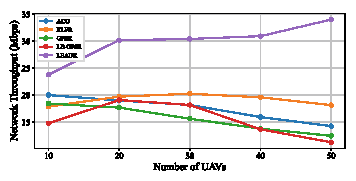
\includegraphics[width=0.49\textwidth]{figures/rq1/num_a.pdf}}\hfill
\subfigure[数据包丢失率\label{rq1:fig:size_b}]{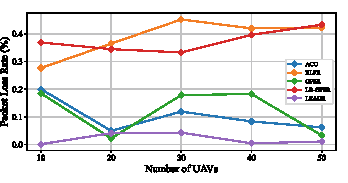
\includegraphics[width=0.49\textwidth]{figures/rq1/num_b.pdf}}
\par\medskip
\subfigure[能量均衡指标\label{rq1:fig:size_c}]{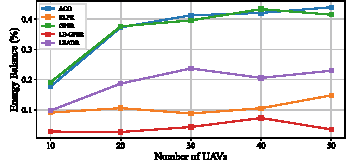
\includegraphics[width=0.49\textwidth]{figures/rq1/num_c.pdf}}\hfill
\subfigure[网络生命周期\label{rq1:fig:size_d}]{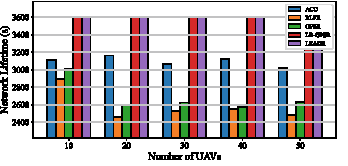
\includegraphics[width=0.49\textwidth]{figures/rq1/num_d.pdf}}
\bicaption{不同无人机数量下的路由性能比较}{Routing performance with different numbers of UAVs}
\label{rq1:fig:size}
\end{figure}

从图~\ref{rq1:fig:size_a} 可以看出，在全部五种规模下，LEADR 的聚合吞吐量均位居首位，且整体随节点数增多而稳步抬升；相比之下，GPSR 与 ACO 整体呈下滑趋势，LB-GPSR 先升后降，RLFR 则在中等规模后明显回落。原因在于，GPSR 等策略过度依赖单一地理指标，节点增多后流量仍易扎堆于少数位置有利的中继并引发局部拥塞；LB-GPSR 虽能靠轮询打散流量，却忽视了各链路信道质量的悬殊差异。而 LEADR 借助队列权重拉升积压节点的发送优先级，配合闭式功率控制与邻居电量修正，既能充分吸纳新增中继，又能防止热点过载。图~\ref{rq1:fig:size_b} 进一步印证了这一点：LEADR 的丢包率始终压制在低位，ACO 和 GPSR 随规模波动较大，LB-GPSR 与 RLFR 则始终维持较高丢包。

在能量维度上，图~\ref{rq1:fig:size_c} 显示 LEADR 的能量离散度低于 ACO 和 GPSR，但略高于 LB-GPSR 与 RLFR，且随规模有所起伏。这符合设计预期——LEADR 并不强行拉平各节点耗电，而是允许处于高吞吐位置且链路条件好的节点承担更多转发量。即便如此，由图~\ref{rq1:fig:size_d} 可见，LEADR 与 LB-GPSR 均在五种规模下撑满了 $3600\,\mathrm{s}$ 的完整任务周期，而其他三种基线均提前出现了节点耗尽的情况。在同样满足续航要求的两种策略中，LEADR 换来了高得多的有效吞吐和显著更低的丢包率。

\subsection{通信范围的影响}
\label{rq1:sec:experiment_range}

第二组实验固定 30 架无人机，将最大通信半径由 $200\,\mathrm{m}$ 以 $25\,\mathrm{m}$ 为步长增至 $300\,\mathrm{m}$。增大通信范围会增加单跳可达邻居数、缩短多跳路径长度，但同时也放大了并发干扰范围，测试结果见图~\ref{rq1:fig:range}。

\begin{figure}[!htbp]
\centering
\subfigure[网络聚合吞吐量\label{rq1:fig:range_a}]{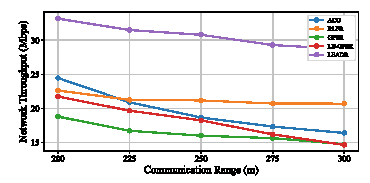
\includegraphics[width=0.49\textwidth]{figures/rq1/com_a.pdf}}\hfill
\subfigure[数据包丢失率\label{rq1:fig:range_b}]{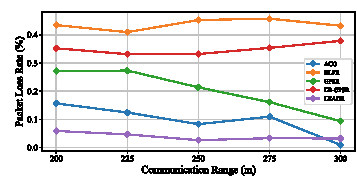
\includegraphics[width=0.49\textwidth]{figures/rq1/com_b.pdf}}
\par\medskip
\subfigure[能量均衡指标\label{rq1:fig:range_c}]{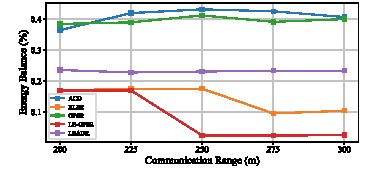
\includegraphics[width=0.49\textwidth]{figures/rq1/com_c.pdf}}\hfill
\subfigure[网络生命周期\label{rq1:fig:range_d}]{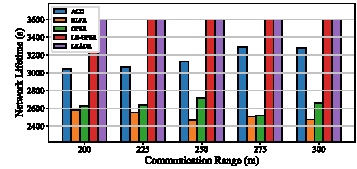
\includegraphics[width=0.49\textwidth]{figures/rq1/com_d.pdf}}
\bicaption{不同通信范围下的路由性能比较}{Routing performance under different communication ranges}
\label{rq1:fig:range}
\end{figure}

由图~\ref{rq1:fig:range_a} 可见，随着通信范围扩大，各算法的聚合吞吐量整体呈下降态势，而 LEADR 始终保持最高水平且降幅最为平缓。这里需要结合指标定义理解：聚合吞吐量累计的是各跳转发服务之和，通信半径增大使得许多数据无需过多中继即可送达中心，跳数减少自然会拉低累计转发计数；同时，拉长单跳距离与扩大干扰域也会压低单跳速率。因此，评价不同通信范围下的转发表现必须结合丢包率来看。图~\ref{rq1:fig:range_b} 表明，LEADR 在所有半径下均维持了最低丢包，大通信范围时几乎趋近于零；ACO 和 GPSR 随连通性改善有所下降，而 LB-GPSR 与 RLFR 的丢包依然偏高。这是因为远距离直连邻居虽然减少了跳数，却往往伴随严重的路径损耗，LEADR 先按当前干扰与距离求解最优功率收益，再综合邻居电量选路，避免了盲目选择远距离低效链路。

能量方面（图~\ref{rq1:fig:range_c}、\ref{rq1:fig:range_d}），LEADR 的能量离散度随通信范围变化保持平稳，仍低于 ACO 和 GPSR、高于中大范围下的 LB-GPSR 及 RLFR；同时与 LB-GPSR 一道在全部五组配置中维持了 $3600\,\mathrm{s}$ 的完整生命周期，而其余基线的寿命并未随通信范围扩大实现单调增长。

\subsection{飞行速度的影响}
\label{rq1:sec:experiment_speed}

第三组实验将无人机平均飞行速度从 $5\,\mathrm{m/s}$ 提升至 $25\,\mathrm{m/s}$。速度加快虽会加剧邻居更替频率，但也为原本受限于局部位置的热点流量提供了动态转移机会，结果如图~\ref{rq1:fig:speed} 所示。

\begin{figure}[!htbp]
\centering
\subfigure[网络聚合吞吐量\label{rq1:fig:speed_a}]{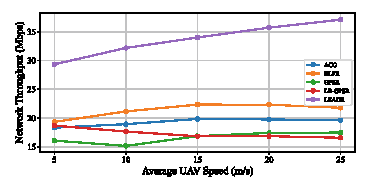
\includegraphics[width=0.49\textwidth]{figures/rq1/speed_a.pdf}}\hfill
\subfigure[数据包丢失率\label{rq1:fig:speed_b}]{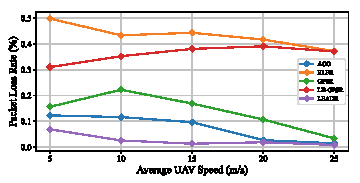
\includegraphics[width=0.49\textwidth]{figures/rq1/speed_b.pdf}}
\par\medskip
\subfigure[能量均衡指标\label{rq1:fig:speed_c}]{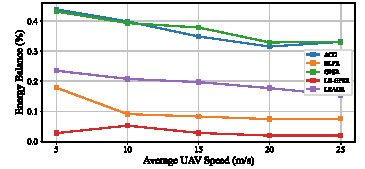
\includegraphics[width=0.49\textwidth]{figures/rq1/speed_c.pdf}}\hfill
\subfigure[网络生命周期\label{rq1:fig:speed_d}]{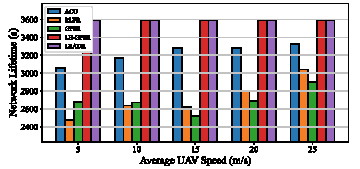
\includegraphics[width=0.49\textwidth]{figures/rq1/speed_d.pdf}}
\bicaption{不同平均飞行速度下的路由性能比较}{Routing performance at different average UAV speeds}
\label{rq1:fig:speed}
\end{figure}

从图~\ref{rq1:fig:speed_a} 与图~\ref{rq1:fig:speed_b} 可以看到，随着飞行速度提高，LEADR 的吞吐量持续攀升并稳居第一，丢包率则同步走低，在高速场景下接近于零；ACO 和 RLFR 吞吐增幅有限，GPSR 在中速段出现波动，LB-GPSR 甚至整体走低。究其原因，机械轮询无法及时感知邻居链路的瞬时变化，而 LEADR 一方面通过自适应 HELLO 缩短高速下的状态刷新周期，确保新出现的优质链路第一时间进入候选，另一方面持续依据累计能耗与预算偏差动态修正权重，防止节点短暂进入有利位置时被过度透支。

在能量与寿命方面（图~\ref{rq1:fig:speed_c}、\ref{rq1:fig:speed_d}），高速移动让更多节点轮流经过有利转发区域，因而 LEADR 与多个基线的能量离散度均有所下降。网络生命周期上，LEADR 在全部五档速度下均达到 $3600\,\mathrm{s}$；反观 LB-GPSR 在 $5\,\mathrm{m/s}$ 低速热点持续存在的条件下未能撑满完整窗口，其余基线则随速度波动。这说明 LEADR 既能在低速热点期保住关键节点续航，又能在高速动态拓扑中充分挖掘新增路径收益。

综合三组仿真结果来看，在节点规模、通信半径与移动速度大幅变化的情况下，LEADR 均能覆盖完整任务周期并取得最高的聚合吞吐与最低的丢包率。同时，其能量离散度高于 LB-GPSR 和 RLFR 的现象也揭示了一个实际权衡：在通信能量受限的多跳网络中，与其强求各节点消耗绝对均等，不如依据位置、信道效率与剩余电量动态分配负载，才能在守住续航底线的前提下最大化网络有效转发能力。

\section{本章小结}

本章面向有限通信能量约束下的无人机多跳回传问题，提出了分布式路由与功率联合控制方法 LEADR。该方法借助李雅普诺夫漂移加惩罚机制，将数据队列积压、累计能耗及虚拟能量队列统一纳入本地决策目标，在固定观测干扰下求得链路发射功率的闭式解；同时结合邻居剩余电量与地理进度筛选下一跳，并利用相对运动预测自适应调整 HELLO 广播间隔，使单节点决策保持线性复杂度。多场景仿真结果表明，LEADR 在不提前耗尽节点电量的前提下，显著优于各对比基线，保持了高聚合吞吐与低丢包率。